\chapter{Related and Existing Work}
\label{chap:Related and Existing Work}

This chapter serves two purposes.
First we will discuss existing solutions.
The differences between these and our proposed work will serve to highlight in what ways our work expands existing solutions.
Then we will take a look at the academic side of file synchronization and discuss related papers.
These will serve as a foundation for how we implement the Tinzenite protocol.

\section{Existing Software}
\label{sec:Existing Software}

\begin{figure}[htp]
\centering
    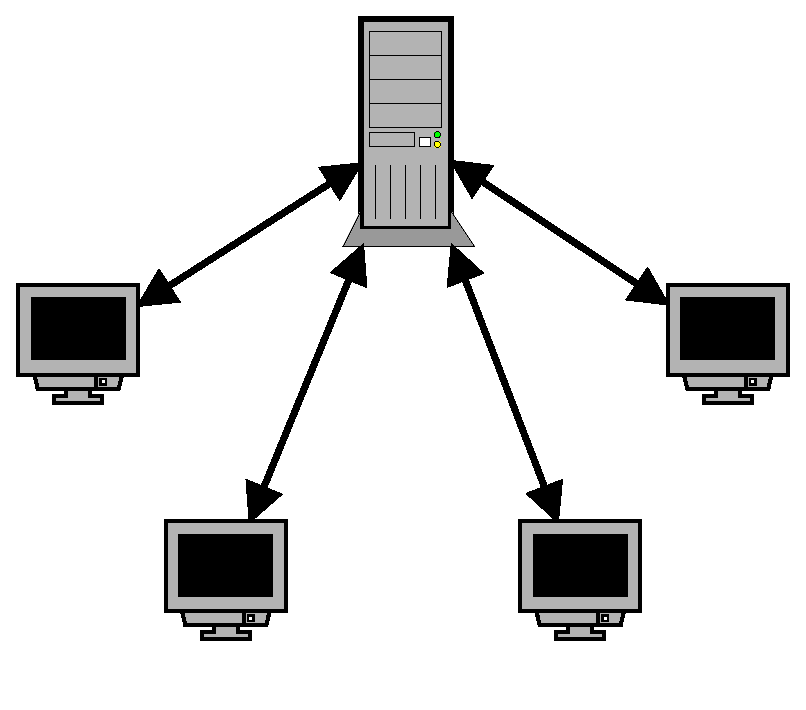
\includegraphics[width=0.3\linewidth]{diagram/topo_s2c}
    \hspace{2em}
    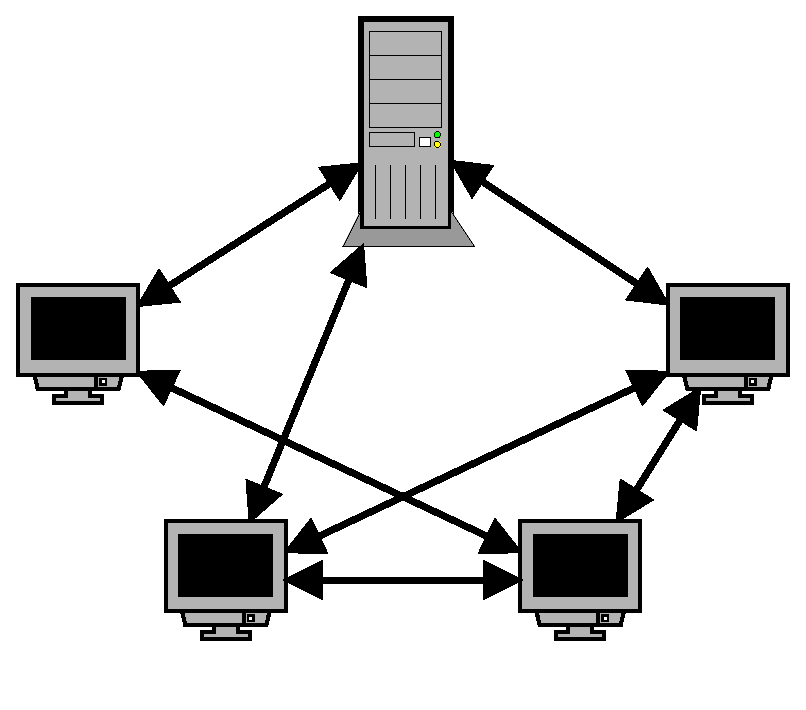
\includegraphics[width=0.3\linewidth]{diagram/topo_p2p}
\caption[Example Network Structures]{Example diagrams of a server client architecture (left) and a peer to peer architecture (right). Note that the peer to peer architecture does not exclude servers as peers.}
\label{fig:example_netarch}
\end{figure}

For any internet technology there are two options for how to structure its architecture in general.
Most of the internet today is cleanly divided in a client-server structure where a client always requests information from a central server.
This is a strongly hierarchical structure.
An example of this is downloading a PDF from a website.
The other option is a distributed peer to peer model, where a client requests information from any other client and in turn will also respond to queries from other clients.
One of the more well known candidates of this is the Bittorrent protocol~\cite{web:site:bittorrent}.
Both options have been used in existing file synchronization solutions.
See figure~\ref{fig:example_netarch} for an example diagram of the two architectures.
Therefore we have divided the existing software we will shortly discuss in the following sections between these two extremes.

\subsection{Client-Server Solutions}
\label{sub:Client-Server Solutions}

For client-server solutions any user must rely on the availability of the central server.
These are often hosted by third parties in a distributed manner for reasons of performance and scaling.
Providing a central service that is required for the file synchronization to work also allows easy monetization.
Since a large amount of such services exist, we will highlight only the three most popular ones for this thesis.
These are respectively: Dropbox with 300 million users, Microsoft's OneDrive with 250 million users, and Google Drive with 240 million users as of 2014~\cite{web:site:fortune}.

\subsubsection{Dropbox}
\label{subs:Dropbox}

Dropbox~\cite{web:site:dropbox} is one of the most popular cloud storage providers currently and is known by many users looking for a solution that works across multiple operating systems.
Positive features include web access to stored data, clients for many different platforms, easy sharing of data with outsiders, and ease of use.
On the negative side the service relies on its back-end servers, although computers can synchronize files between themselves on a local area network.
Dropbox also lacks any end to end encryption, but does encrypt data while in transit and when "at rest" in their data centers~\cite{web:site:dropbox:blog}.
Therefore it comes with little surprise that they were prominently featured in the Snowden leaks~\cite{web:site:rt:dropbox}.
The company does have full access to any data the user uploads to their servers, as long as the users do not encrypt the files beforehand themselves.
Therefore we can extrapolate that Dropbox can offer up a user's data if required to by a fourth party, as is the case in the United States of America.

Dropbox offers a free account for a basic storage plan.
Additional storage capacity is available for purchase.
None of the core applications have been open sourced to date, meaning even if Dropbox implemented strong encryption it could not be independently verified.

\subsubsection{OneDrive}
\label{subs:OneDrive}

With the release of Microsoft's newest operating system the company has increased its push for public adoption of its OneDrive~\cite{web:site:onedrive} cloud storage service.
It is now directly integrated within Windows 10 and is opt-out for users that do not wish to utilize it.
OneDrive is integrated with Microsoft's answer to Google Docs, Office 365.
Furthermore more free storage is added for registering devices and using Microsoft's products.

Similar to its two competitors, the base plan is free, with the option of paying monthly for an increase in storage space.
No software for OneDrive has been open sourced.

\subsubsection{Google Drive}
\label{subs:Google Drive}

Google Drive~\cite{web:site:gdrive} is similar to Dropbox in term of its functionality.
It does go a step further than Dropbox by integrating tightly with their suite of online applications for creating and editing documents, named Google Docs.
Google also has full access to all data that users upload to their servers.
This in turn means that under the PRISM program by the NSA, all such data is also retrievable by a fourth party~\cite{web:site:rt:google}.

Google also offers a basic storage amount at no charge for the user.
Again additional space can be purchased on a monthly basis.
Apart from offering access to fewer clients than Dropbox, Google also has failed to open source the components of its service.

\subsection{Peer to Peer Solutions}
\label{sub:Peer to Peer Solutions}

Peer to peer systems work without a central server.
The trade off is that such solutions require assistance in locating other peers, which means that some form of a peer discovery system must be implemented.
While this could be done via a central server, nowadays the common solution to the problem is a distributed hash table~\cite{ratnasamy2001scalable} which is used to look up the required peers.
Once another peer has been found the connection can be established.
Apart from not relying on the availability and trustworthiness of a central server, peer to peer solutions offer a possible performance advantage as they can distribute bandwidth between every peer, even actively unchoke a saturated peer.
As an added bonus the path data takes between two peers will always be the most direct path as no data must first go towards a third party.
This bonus can be lost if onion routing is implemented for anonymity purposes.

\subsubsection{BitTorrent Sync}
\label{subs:BitTorrent Sync}

An existing solution for a peer to peer data synchronization service is Sync~\cite{web:site:bittorrent_sync} from the BitTorrent company.
It is built on existing Bittorrent technology and thus keeps many of the positive features associated with torrents: reducing the impact of transferring large files over a limited network.
Therefore it has no central point of failure and can even run without internet access by transferring files between computers on a local area network directly.
However, just as the client-server solutions before, Sync is closed source.

Clients exist for a multitude of platforms.
While information is encrypted in transfer, there is no differentiation for untrusted clients.
Sync is free for basic usage, but requires a paid account for additional features that offer more fine grained control.

\subsubsection{Syncthing}
\label{subs:Syncthing}

Syncthing~\cite{web:site:synthing} is an open source file synchronization software on an equally free block exchange protocol.
This protocol is a mixed data transfer and communication protocol in one, with encryption for all communication built in directly.
Again the user can not designate untrusted peers.

Unlike the other solutions mentioned here, Syncthing is open source and can thus be independently verified to be secure.
Like Tinzenite it is also implemented in Golang.
The downside is that Syncthing lacks a feature which BitTorrent Sync shares with most client-server solutions: the capability of sharing a specified file or directory with other users who are not part of the storage system.

\subsection{Additional Security Layers}
\label{sub:Additional Security Layers}

It is of course possible to encrypt all data before using any data storage service beforehand.
This has a few notable downsides however.
For many client-server solutions the user loses out on web access to the data along with a host of additional feature built on the availability of the data.
While advanced users may be capable of encrypting their data themselves using a range of available tools, such solutions require the user to manage the encryption keys themselves.
This is a non trivial issue beyond adding an additional hurdle to using data storage services.
As so often commercial solutions for this exist.

\subsubsection{Boxcryptor}
\label{subs:Boxcryptor}

All three server-client services mentioned are not to be trusted with private information that must remain secure due to possible fourth party access.
However solutions for encrypting the data sent over such services which manage the encryption keys exist.
One example of such a service is the Boxcryptor software~\cite{web:site:boxcryptor}.
It encrypts all data before uploading it to the connected cloud storage service and decrypts it when retrieving it.
The user keys are attached to the user's account.
Asymmetric encryption is used to upload all keys to the companies key server so that other clients can retrieve and, with a correct password, decrypt the data.
Sharing of data is still possible even for users without an account by utilizing special keys.

The downside to this approach is mainly that it has to be used on top of an existing cloud storage service.
This effectively means that the user must run an additional program on top of the file storage service to ensure secure data.
Boxcryptor can be used with most existing third party data storage systems.
Boxcryptor offers a free version of its service, but to access all security features a paid subscription is required.
The software is not open source and thus not independently verifiable.

\subsection{Comparison}
\label{sub:Comparison}

In this section we will briefly highlight the capabilities and differences between the discussed existing solutions.
We chose to compare the features that we believe to be most important to this thesis.
See table~\ref{table:software_comparison}.

\begin{table}[htp]
\begin{threeparttable}
\centering
\begin{tabulary}{\textwidth}{ p{2.8cm} || c | C | C | C | C }
    \textbf{Name} & \textbf{Architecture} & \textbf{Free Storage} & \textbf{Client-side Encryption} & \textbf{Open Source} & \textbf{Account Required} \\
    \hline \hline
    Dropbox & Centralized & 2 GB & & & \checkmark \\
    \hline
    OneDrive & Centralized & 15 GB & & & \checkmark \\
    \hline
    Google Drive & Centralized & 15 GB & & & \checkmark \\
    \hline
    Boxcryptor & --\tnote{a} & --\tnote{b} & \checkmark & & \checkmark \\
    \hline
    BitTorrent Sync & Distributed & $\infty$ & & & \checkmark \\
    \hline
    Syncthing & Distributed & $\infty$ & & \checkmark & \\
\end{tabulary}
\scriptsize{
\begin{tablenotes}
    \item[a] Boxcryptor is used on top of an existing cloud storage provider.
        The encryption infrastructure itself is centralized.
    \item[b] Boxcryptor is free to use but many features are only available for a paid account.
\end{tablenotes}
}
\end{threeparttable}
\caption[Existing Software Comparison]{This table serves to highlight the differences between the existing software previously discussed.}
\label{table:software_comparison}
\end{table}

\section{Papers}
\label{sec:Papers}

The following discussion concerns papers that we believe have an impact on our work.
We discuss their general content with a focus on what information we extracted and how we believe we can apply it to Tinzenite.

\subsection{What is a File Synchronizer?}
\label{sub:What is a File Synchronizer?}

The paper by Balasubramaniam and Pierce~\cite{balasubramaniam1998file} has the stated goal of offering a framework for describing the behavior of file synchronizers.
Notably the paper's authors divide the process into two separate phases: update detection and reconciliation.
Update detection is defined as the recognition of where updates have been made to the directory since the last synchronization.
Reconciliation is defined as the combination of updates between peers to transfer all peers to a new, synchronized state.

For Tinzenite we assimilated a few things out of this paper: primarily the distinction between the update detection and the reconciliation phase.
We will also initially ignore links and file permissions due to increased complexity, but unlike them we will never modify a file ourself.
The paper also gave us a definition for the type of update detection strategy we wanted to try: namely the modtime inode strategy.
Ideally we would take an on-line update detector but this seems impossible to do under Linux currently for an unlimited amount of files.
Also of interest is the differentiation between pull and push models for propagating updates.
Tinzenite intends to be a hybrid between the two: while the main work will be done via push -- once peers have established a connection -- updates may also be propagated via pull for performance reasons.
In the reconciliation section of the paper is the listing of the various possible states that two replicas of a directory can possibly reach given a set of operations, which is also of interest for this thesis.
We intend to ensure that the core protocol for Tinzenite will be capable of handling all of them to the best of its abilities.

\subsection{An Algebraic Approach to File Synchronization}
\label{sub:An Algebraic Approach to File Synchronization}

The paper by Ramsey and Csirmaz~\cite{ramsey2001algebraic} presents an algebra for reasoning about file system operations with the intended purpose of specifying an algorithm for file synchronization.
Interesting for our work is the discussion of possible commands that can be executed on said file algebra.
While from a user's point of view a multitude of operations seems possible (create, remove, rename, move, derive, and edit) the paper's authors distill these down to just three for the technical side: create, remove, and edit.
Rename can be executed by removing the original file and creating a new file with the new name while keeping the content identical.
Move can be executed much the same but keeps the name, instead changing the location where the new file is created.
Derive is argued to be indistinguishable from edit without higher level knowledge.
While not impossible to detect, this feature we consider to be beyond the scope of Tinzenite.
Features that Tinzenite shares with the paper's prototype include that parents must be created before their children and that children must be removed before their parents.

The paper also offers a number of improvements that Tinzenite could incorporate.
Notably this includes support for an explicit move command.
This would remove the need for removing and recreating a file's content when it was moved, thus making this operation more performant.% performant is written correctly
They also suggest using fingerprints of content to avoid sending data that already exists.
Tinzenite already utilizes content hashes, so expanding it to be more intelligent about when to request actual data to be sent should be easily implementable by comparing hashes of files before requesting transfers.

\subsection{Peer-to-Peer Reconciliation Based Replication for Mobile Computers}
\label{sub:Peer-to-Peer Reconciliation Based Replication for Mobile Computers}

In~\cite{reiher1996peer}, Reiher et al. nicely state the benefits and drawbacks of using a peer to peer system for file synchronization in regard to mobile devices.
Benefits include not having to rely on an permanently available server, being able to transfer files without access to a central server, and transferring files over the shortest available network path.
The authors list as drawbacks the higher required complexity of the algorithms used to control the replication.
They conclude that peer to peer replication is well suited for mobile devices.

\subsection{Perspectives on Optimistically Replicated, Peer-to-Peer Filing}
\label{sub:Perspectives on Optimistically Replicated, Peer-to-Peer Filing}

The paper by Page et al.~\cite{page1998perspectives} is notable in our case for two main reasons.
It offers a nice set of definitions of problems that we must also solve for Tinzenite and even offers relevant solutions.
The authors also discuss the performance of their implementation.
Focus of the paper is the evaluation of the use of optimistic replica consistency, automatic update conflict detection and repair, the peer to peer interaction model, and the Ficus design and construction.

Relevant for Tinzenite is the paper's solution to the insert delete ambiguity.
The solution is to keep a list of deletions until all peers know of the deletion.
Only then can the deletion actually be garbage collected.
In Tinzenite we will use a similar approach.

\section{Conclusion}
\label{sec:Conclusion}

Based on the listed existing solutions and the briefly discussed related papers we have synthesized a set of features that we wish Tinzenite to have.
These will be discussed in the next chapter.
More importantly our research highlights a few problems that we will need to solve or use already existing solutions for.
This starts with defining the operations we will allow on objects within a directory and continue on to how to solve ambiguities and merge conflicts when synchronizing between multiple peers.
